\chapter{Agenda tříd}
\section{Popis problému}
Implementace agendy tříd v~rámci školního informačního systému (dále jen ŠIS) vyžaduje pečlivé zvážení administrativních i~technických aspektů správy školy.~Systém musí efektivně zpracovat evidenci tříd a~žáků, rozvrhy a~mimořádné rozvrhy.~Současně umožňovat uchovávání dat pro administrativní či právní důvody.~Je nezbytné zajistit konzistenci dat napříč různými časovými obdobími a~umožnit flexibilní reakce na změny, jako jsou přechody žáků mezi třídami, opakování ročníků nebo přerušení studia.

Cílem je navrhnout a~implementovat systém, který bude nejen efektivní a~flexibilní, ale také splní všechny požadavky na správu tříd a~souvisejících dat.~V~následujících částech jsou jednotlivé návrhy konzultovány s~jejich dopady na celkovou konzistenci a~funkčnost ŠIS.

\section{Požadavky}
V~kontextu školního rozvrhového systému představuje agenda tříd komplexní správu informací o~třídách, která zahrnuje nejen udržování aktuálních seznamů tříd a~jejich žáků, ale také systematické řízení veškerých změn v~průběhu studia. Systém musí být schopen efektivně manipulovat s~údaji o~žácích, což zahrnuje ukládání a~aktualizaci jejich základních informací, jako je i~přesné zaznamenávání a~sledování změn v~jejich studijním procesu. To zahrnuje přechody žáků mezi třídami, opakování ročníku v~důsledku neprospěchu či přestupy na jiné školy.

Implementace takové funkcionality je nezbytná pro zajištění správného a~podpůrného vzdělávacího procesu, který respektuje individuální potřeby žáků a~podporuje jejich všestranný rozvoj. Efektivní správa těchto změn přispívá k~vytvoření příznivého vzdělávacího prostředí, ve kterém se žáci mohou soustředit na svůj růst bez obav z~administrativních překážek spojených se změnami ve studiu.

Jako klíčové systémové požadavky na implementaci je považováno:
\begin{enumerate}
    \item \textbf{Konzistence dat:}\label{req-data-consistency} zajištění, že informace o~třídách, rozvrzích a~žácích jsou konzistentní napříč různými časovými obdobími;
    \item \textbf{Historická data:}\label{req-historical-data} uchovávání historických záznamů pro administrativní a~právní účely;
    \item \textbf{Flexibilita:}\label{req-flexibility} schopnost systému pružně reagovat na změny, jako jsou vertikální či horizontální přechody žáků, změny učitelů či učeben.
    \item \textbf{Optimalizace:}\label{req-optimization} Systém by měl být optimalizován pro výkon a~efektivitu, zajišťující rychlý přístup k~datům  a~efektivní využití zdrojů, jako jsou paměť a~výpočetní výkon.
    \item \textbf{Horizontální přechody žáků:}\label{req-horizontal-student-move} Žák může během studia, za specifických podmínek stanovených školským zákonem a~na povolení ředitele školy, změnit třídu, obor nebo školu. 
    \item \textbf{Vertikální přechody žáků:}\label{req-vertical-student-move} Žák, který nesplní zákonné požadavky pro postup do dalšího ročníku (neprospěje), může být v~následujícím školním roce zařazen do jiné třídy a~ročník opakovat.~Žák též může studium přerušit, či úplně ukončit.
    \item \textbf{Přerušení studia:}\label{req-cancel-student-move} Žák může během probíhajícího studia požádat ředitele školy o~přerušení vzdělávání.~Maximální doba trvání přerušení dle zákona §~66 odst.~5 zákona č.~561/2004 Sb.~(školský zákon) ve znění od 1. ledna 2024\cite{skolsky-zakon-preruseni-obyc} až na dobu dvou let, s~výjimkou mateřství\cite{skolsky-zakon-preruseni-materstvi}, které se řídí odlišným postupem.
    \item \textbf{Administrativní a~kontrolní požadavky:}\label{req-backups} Uchovávání dat pro administrativní, právní a~jiné důvody jako jsou komunikace se státními orgány nebo například soudy.
\end{enumerate}

V~následujících částech této kapitoly jsou podrobněji zmíněny jednotlivé návrhy implementace a~jejich dopady na celkovou konzistenci a~funkčnost systému.

\section{Návrhy implementace}
Na základě výše uvedených požadavků a~kontextu jsou navrženy tři hlavní přístupy k~implementaci agendy tříd. Dalšími kroky bude správně přiřadit správu žákovských skupin, třídní knihy, rozvrhu a~žákovských absencí.

\begin{enumerate}
    \item \textbf{Ukládání pouze aktuálního ročníku:} Tento přístup uchovává na serveru informace pouze o~aktuálním ročníku a~data z~minulých let jsou uložena na odděleném serveru.

    \begin{figure}[H]
        \centering
        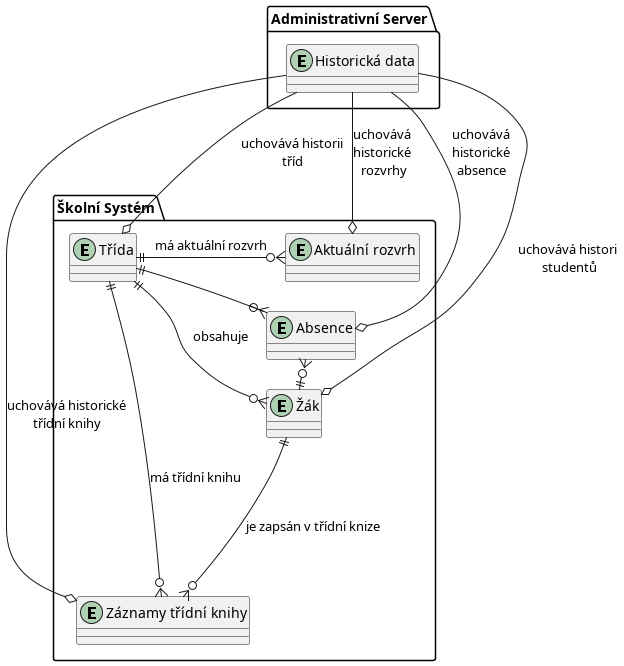
\includegraphics[width=.8\textwidth]{ed-schedule-only-actual.png}
        \caption{Diagram varianty s~ukládáním pouze aktuálního ročníku a~aktuálních rozvrhů}
        \label{fig:ed-schedule-only-actual}
    \end{figure}
    
    Před začátkem každého školního roku by bylo nezbytné provést synchronizační proces, který by zahrnoval archivaci stávajících dat na samostatný server, odstranění neaktuálních dat z~rozvrhového serveru a~nahrání nových dat. Tento přístup má následující výhody a~nevýhody ve vztahu k~definovaným požadavkům:

    \textbf{Výhody:}
    \begin{itemize} 
        \item \textbf{Snížení datové zátěže:} Uchovávání pouze aktuálních dat snižuje nároky na úložný prostor a~výpočetní výkon díky menšímu objemu dat. Tento aspekt podporuje \textbf{optimalizaci systému}~(\ref{req-optimization}), neboť umožňuje rychlejší přístup k~datům a~efektivnější využití zdrojů.

        \item \textbf{Zjednodušená správa aktuálních dat:} Práce pouze s~aktuálními daty usnadňuje správu a~údržbu systému, neboť není nutné řešit historické záznamy v~běžném provozu. To může zvýšit produktivitu administrativního personálu a~přispět k~\textbf{optimalizaci}~(\ref{req-optimization}) z~hlediska provozní efektivity.
    \end{itemize}

    \textbf{Nevýhody:}
    \begin{itemize} 
        \item \textbf{Složitost synchronizačního procesu:} Synchronizace mezi servery může být náročná na implementaci a~vyžaduje důkladné plánování a~testování. Chyby v~tomto procesu mohou vést k~nekonzistenci dat nebo jejich ztrátě, což ohrožuje \textbf{konzistenci dat}~(\ref{req-data-consistency}) a~může negativně ovlivnit \textbf{optimalizaci}~(\ref{req-optimization}) kvůli zvýšeným nárokům na správu.

        \item \textbf{Riziko nenávratné ztráty dat:} V~případě chyby během synchronizace hrozí nenávratná ztráta klíčových dat, což může mít závažné právní a~administrativní důsledky. To nesplňuje požadavky na \textbf{uchovávání historických dat}~(\ref{req-historical-data}) a~\textbf{administrativní a~kontrolní požadavky}~(\ref{req-backups}).

        \item \textbf{Obtížnější přístup k~historickým datům:} Oddělení historických dat na jiný server může komplikovat jejich dostupnost při potřebě rychlého získání informací, například během inspekcí nebo právních řízení. To omezuje \textbf{flexibilitu systému}~(\ref{req-flexibility}) a~může zpomalit reakce systému, což má negativní dopad na \textbf{optimalizaci}~(\ref{req-optimization}) z~hlediska rychlosti přístupu k~datům.

        \item \textbf{Zvýšené nároky na personální zdroje:} Správa dvou samostatných serverů může vyžadovat více lidských zdrojů a~koordinaci mezi týmy, což zvyšuje provozní náklady a~může komplikovat administrativní procesy. To může negativně ovlivnit \textbf{optimalizaci}~(\ref{req-optimization}), neboť zvyšuje celkovou složitost systému.

        \item \textbf{Omezení flexibility:} Tento přístup může omezit schopnost systému rychle reagovat na změny zasahující do minulých let, jako je \textbf{přerušení studia}~(\ref{req-cancel-student-move}), \textbf{vertikální přechody žáků}~(\ref{req-vertical-student-move}) a~\textbf{horizontální přechody žáků}~(\ref{req-horizontal-student-move}). Nesplňuje tedy požadavek na \textbf{flexibilitu systému}~(\ref{req-flexibility}).
    \end{itemize}

    \textbf{Shrnutí:}
    
    Přestože tento přístup nabízí výhody v~podobě snížení datové zátěže a~může přispět k~\textbf{optimalizaci}~(\ref{req-optimization}) z~hlediska efektivního využití zdrojů pro aktuální data, výrazně nesplňuje klíčové systémové požadavky na \textbf{konzistenci dat}~(\ref{req-data-consistency}), \textbf{uchovávání historických dat}~(\ref{req-historical-data}), \textbf{flexibilitu systému}~(\ref{req-flexibility}) a~\textbf{administrativní a~kontrolní požadavky}~(\ref{req-backups}). Rizika spojená s~tímto řešením, zejména možnost ztráty dat a~omezená schopnost systému reagovat na změny v~průběhu studia, převažují nad jeho přínosy. Navíc komplikace spojené se synchronizací a~správou dvou serverů mohou negativně ovlivnit \textbf{optimalizaci}~(\ref{req-optimization}) systému jako celku. To naznačuje potřebu zvážit alternativní přístupy, které lépe naplňují definované požadavky a~zajišťují vyšší úroveň spolehlivosti, efektivity a~optimalizace systému.

    \item \textbf{Třída s~vypočteným ročníkem:} Tento přístup ukládá informace o~třídách pomocí kombinace prefixu, suffixu a~data vytvoření třídy.~Ročník je vypočten jako rozdíl mezi datem vytvoření třídy a~začátkem aktuálního školního roku. Příkladem prefixu může značka oboru, zatímco sufix může rozlišovat jednotlivé třídy ve stejném ročníku.

    \begin{figure}[H]
        \centering
        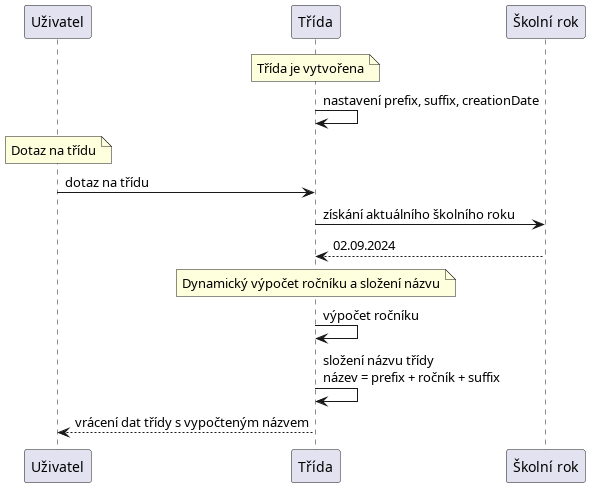
\includegraphics[width=\textwidth]{td-schedule-calculated-class.png}
        \caption{Schéma průběhu dotazu na jméno třídy}
        \label{fig:td-schedule-calculated-class}
    \end{figure}
    
    Hlavním problémem tohoto přístupu je samotný výpočet ročníků. Aby byla zajištěna aktuálnost dat, měl by být ročník vždy vypočítáván dynamicky, neboť jakákoli forma uchovávání mezivýsledků by mohla vést k~nekonzistenci v~čase. Při požadavku na získání aktuálních tříd musí server vypočítat ročníky pro všechny třídy a~sestavit jejich plné názvy, což může zatěžovat systém a~zvyšovat latenci odpovědi.Tento aspekt může negativně ovlivnit \textbf{optimalizaci systému}~(\ref{req-optimization}), neboť zvyšuje výpočetní nároky a~může zpomalit odezvu systému.

    Jednou s~možných variant optimalizace je uchovávání vypočtených názvů tříd v~mezipaměti (cache) s~událostmi řízenou invalidací. Mezipaměť by byla invalidována při manipulaci se třídami nebo při přechodu do nového školního roku. Tato strategie však přináší další složitost systému a~může komplikovat jeho údržbu, což může ovlivnit \textbf{optimalizaci}~(\ref{req-optimization}).

    Dalším významným problémem tohoto řešení jsou vertikální a~horizontální přechody žáků mezi třídami nebo změny ve studiu během školního roku. V~případě, kdy žák přestupuje mezi třídami vertikálně nebo horizontálně, nastávají tři možné varianty řešení:
    \begin{itemize}
        \item \textbf{Odebrání žáka z~aktuální třídy a~přiřazení do nové třídy:} Tento postup by vedl ke ztrátě historických záznamů, protože třída je jedním z~atributů žáka. Přestože by bylo možné vést záznamy o~změnách, tato metoda nepokrývá všechny požadavky na snadnou manipulaci s~daty a~může způsobit nekonzistenci v~historických údajích, což ohrožuje \textbf{konzistenci dat}~(\ref{req-data-consistency}) a~nesplňuje požadavek na \textbf{uchovávání historických dat}~(\ref{req-historical-data}).

        \item \textbf{Přidání nového žáka, který začíná na škole studovat v~pokročilém ročníku:} Tím by byla zajištěna konzistence dat, avšak vznikly by duplicitní účty pro jednoho žáka.~Řešením může být propojení minulých účtů žáka s~novými prostřednictvím relace 1:N, kde by žák měl uložené své minulé účty. Toto řešení však adresuje spíše důsledek než příčinu problému a~může komplikovat správu uživatelských účtů, což nepodporuje \textbf{flexibilitu systému}~(\ref{req-flexibility}).
        \begin{figure}[H]
            \centering
            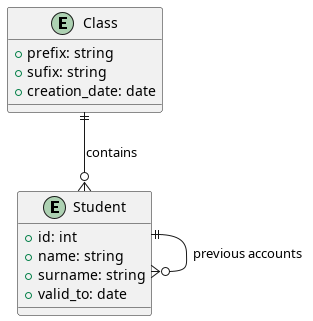
\includegraphics[width=0.5\textwidth]{ed-schedule-calculated-previous-relation.png}
            \caption{Schéma vazby na předchozí účty}
            \label{fig:ed-schedule-calculated-previous-relation}
        \end{figure}

        \item \textbf{Zavedení entity \textit{Studium}, která definuje žákův průchod třídami v~jednotlivých školních letech:} V~tomto přístupu je zavedena nová entita \textit{Studium}, která umožňuje detailní sledování studijní historie žáka.~Školní rok je také reprezentován jako samostatná entita, aby bylo možné přesně zaznamenat období studia.
    \end{itemize}
    \textbf{Zavedení entity \textit{Studium}:}

    Třetí varianta představuje robustní řešení problému sledování studijního postupu žáků. Zavedení entity \textit{Studium} umožňuje:

    \begin{itemize}
        \item \textbf{Detailní sledování historie studia:} Každý záznam v~entitě \textit{Studium} by obsahoval informace o~žákovi, třídě a~školním roce. Tím je možné přesně sledovat, ve které třídě a~v~jakém období žák studoval, což naplňuje požadavky na \textbf{konzistenci dat}~(\ref{req-data-consistency}) a~\textbf{uchovávání historických dat}~(\ref{req-historical-data}).

        \item \textbf{Flexibilní správu změn ve studiu:} Přestupy mezi třídami, opakování ročníků či přerušení studia lze zaznamenat jako nové záznamy v~entitě \textit{Studium}, aniž by docházelo ke ztrátě historických dat nebo nutnosti vytvářet duplicitní účty. To splňuje požadavky na \textbf{flexibilitu systému}~(\ref{req-flexibility}), včetně \textbf{horizontálních}~(\ref{req-horizontal-student-move}) a~\textbf{vertikálních přechodů žáků}~(\ref{req-vertical-student-move}).

        \item \textbf{Lepší integritu dat:} Tento model umožňuje udržet konzistenci a~integritu dat, protože změny jsou evidovány strukturovaně a~je možné je snadno sledovat a~vyhodnocovat. Tím je podpořena \textbf{konzistence dat}~(\ref{req-data-consistency}) a~usnadněno plnění \textbf{administrativních a~kontrolních požadavků}~(\ref{req-backups}).
    \end{itemize}

    \begin{figure}[H]
        \centering
        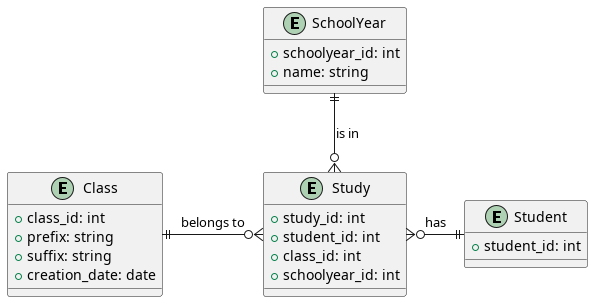
\includegraphics[width=0.8\textwidth]{ed-schedule-calculated-study-entity.png}
        \caption{Schéma s~entitami Studium a~Školní rok}
        \label{fig:ed-schedule-calculated-study-entity}
    \end{figure}

    \textbf{Výhody:}
    \begin{itemize}
        \item Umožňuje přesnou a~kompletní evidenci studijního postupu žáka, což splňuje požadavek na \textbf{uchovávání historických dat}~(\ref{req-historical-data}).

        \item Zajišťuje konzistenci dat bez potřeby vytvářet duplicitní záznamy, což podporuje \textbf{konzistenci dat}~(\ref{req-data-consistency}).

        \item Usnadňuje správu historických dat a~umožňuje flexibilnější reakci na změny ve studiu, čímž se zdá dobrou variantou na požadavek \textbf{flexibility}~(\ref{req-flexibility}).
    \end{itemize}

    \textbf{Nevýhody:}
    \begin{itemize}
        \item \textbf{Zvýšená složitost datového modelu:} Zavedení nových entit (\textit{Studium}, \textit{Školní rok}) zvyšuje komplexitu systému, což může zvýšit náročnost implementace a~správy, a~ovlivnit \textbf{optimalizaci}~(\ref{req-optimization}).

        \item \textbf{Vyšší náročnost databázových dotazů:} Detailnější datový model může vést ke složitějším dotazům a~delší době zpracování, což může negativně ovlivnit výkon systému a~nesplňovat požadavek na \textbf{optimalizaci}~(\ref{req-optimization}).

        \item \textbf{Flexibilita}~(\ref{req-flexibility}) je omezená na celé školní roky. Přesun žáka během roku (například kvůli změně třídního klimatu v~zájmu řešení výchovných opatření) není možný. S~tím jakékoliv jiné úpravy studia během školního roku.

        \begin{figure}[H]
            \centering
            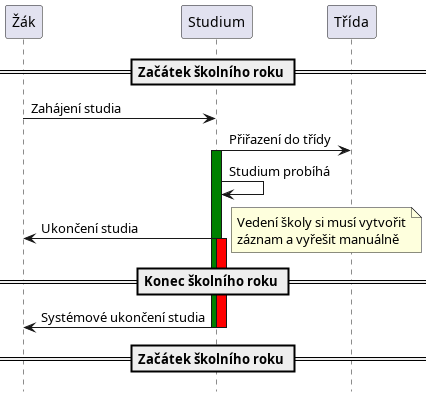
\includegraphics[width=.6\textwidth]{td-schedule-student-run-year-only.png}
            \caption{Schéma průchodu žáka studiem i~s~přerušením na konci školního roku. Zelená část reprezentuje aktivní studium.~Červená část označuje studium, které už není platné, ale systém jej stále eviduje.}
            \label{fig:td-schedule-student-run-year-only}
        \end{figure}
    \end{itemize}

    \textbf{Shrnutí:}
    Tento přístup s~využitím entity \textit{Studium} splňuje klíčové systémové požadavky na \textbf{konzistenci dat}~(\ref{req-data-consistency}), \textbf{uchovávání historických dat}~(\ref{req-historical-data}) a~\textbf{flexibilitu systému}~(\ref{req-flexibility}). Umožňuje efektivní správu \textbf{horizontálních}~(\ref{req-horizontal-student-move}) a~\textbf{vertikálních přechodů žáků}~(\ref{req-vertical-student-move}), jakož i~\textbf{přerušení studia}~(\ref{req-cancel-student-move}). Nevýhodou je zvýšená složitost datového modelu a~možná zátěž na výkon systému, což může ovlivnit \textbf{optimalizaci}~(\ref{req-optimization}). Nicméně, vzhledem k~důležitosti splnění klíčových požadavků je tato varianta považována za vhodnější řešení pro implementaci agendy tříd v~systému.

    \item \textbf{Studium s~datem platnosti:}
    \label{item:class-implementation-from-to-validity} Tento přístup je modifikací předchozího řešení s~implementací entity \textit{Studium}. Modifikací je validační rozsah platnosti studia místo zadání platnosti školního roku.

    \begin{figure}[H]
        \centering
        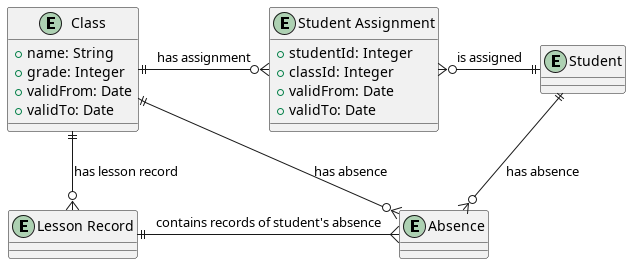
\includegraphics[width=0.8\textwidth]{ed-schedule-validity-from-to.png}
        \caption{Schéma vazby M:N pro validační rozsah studia}
        \label{fig:ed-schedule-validity-from-to}
    \end{figure}

    Tento přístup eliminuje překážky při úpravách studia žáka i~během školního roku. Díky rozsahu platnosti lze například ukončit studium k~určenému dni, což umožňuje přesné zaznamenání změn v~průběhu studia a~splňuje požadavky na \textbf{flexibilitu systému}~(\ref{req-flexibility}) a~\textbf{konzistenci dat}~(\ref{req-data-consistency}). Tento model rovněž usnadňuje správu \textbf{přerušení studia}~(\ref{req-cancel-student-move}) a~\textbf{horizontálních}~(\ref{req-horizontal-student-move}) i~\textbf{vertikálních přechodů žáků}~(\ref{req-vertical-student-move}).

    \textbf{Výhody:}

    \begin{itemize}
        \item \textbf{Flexibilita v~úpravách studia:} Umožňuje přesné zaznamenání začátku a~konce studia žáka, což splňuje požadavek na \textbf{flexibilitu systému}~(\ref{req-flexibility}).
        \item \textbf{Konzistence dat:} Udržuje konzistentní a~přesné záznamy o~studiu žáka, čímž naplňuje požadavek na \textbf{konzistenci dat}~(\ref{req-data-consistency}).
        \item \textbf{Podpora administrativních požadavků:} Detailní záznamy usnadňují splnění \textbf{administrativních a~kontrolních požadavků}~(\ref{req-backups}).
        \item \textbf{Správa přerušení studia:} Umožňuje evidovat \textbf{přerušení studia}~(\ref{req-cancel-student-move}) s~přesným datem začátku a~konce.
    \end{itemize}

    \textbf{Nevýhody:}

    \begin{itemize}
        \item \textbf{Zvýšená složitost datového modelu:} Zavedení rozsahu platnosti studia zvyšuje složitost systému, což může ovlivnit \textbf{optimalizaci}~(\ref{req-optimization}).
        \item \textbf{Vyšší nároky na správu dat:} Detailní evidence může vyžadovat více úsilí při správě a~aktualizaci dat.
    \end{itemize}

    \textbf{Shrnutí:}

    Tento přístup efektivně řeší požadavky na \textbf{flexibilitu systému}~(\ref{req-flexibility}), \textbf{konzistenci dat}~(\ref{req-data-consistency}), a~podporuje správu \textbf{přerušení studia}~(\ref{req-cancel-student-move}), jakož i~\textbf{horizontálních}~(\ref{req-horizontal-student-move}) a~\textbf{vertikálních přechodů žáků}~(\ref{req-vertical-student-move}). Ačkoli zvyšuje složitost datového modelu, výhody spojené s~přesnou evidencí studia a~splněním klíčových požadavků převažují nad nevýhodami.

    \begin{figure}[H]
        \centering
        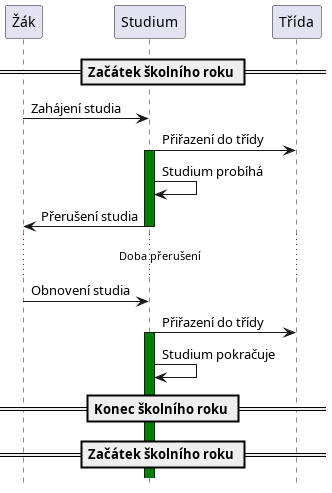
\includegraphics[width=.5\textwidth]{td-schedule-student-run-anytime.png}
        \caption{Schéma průchodu žáka studiem i~s~přerušením ve školním roce. Zelená část reprezentuje aktivní studium.}
        \label{fig:td-schedule-student-run-anytime}
    \end{figure}
\end{enumerate}

\section{Vyhodnocení vhodného řešení}
\begin{landscape}
    \begin{table}[H]
        \centering
        \begin{tabular}{|m{7cm}|m{7cm}|m{7cm}|}
            \hline
            \textbf{Přístup} & \textbf{Výhody (+)} & \textbf{Nevýhody (-)} \\ \hline
            \textbf{Ukládání pouze aktuálního ročníku a~aktuálních rozvrhů} & 1. Minimalizuje datovou zátěž na serveru \newline 2. Jednoduché dotazování na aktuální data & 1. Nutnost synchronizačního mechanismu \newline 2. Riziko ztráty dat při chybě programu \newline 3. Vyžaduje správu od různých zaměstnanců \\ \hline
            \textbf{Třída definována prefixem, suffixem, datem vytvoření a~kalkulovaným ročníkem} & 1. Snížení počtu záznamů v~databázi \newline 2. Flexibilita v~pojmenování tříd & 1. Komplexita kalkulace ročníků \newline 2. Potenciální nekonzistence dat \newline 3. Obtížná manipulace s~propadlými nebo přecházejícími žáky \\ \hline
            \textbf{Třída definována celým názvem a~datem validity od - do} & 1. Konzistence dat při přesunech žáků \newline 2. Jednoduchá správa historických záznamů \newline 3. M:N vazby umožňují flexibilní přiřazení žáků & 1. Vyšší náročnost dotazování na aktuální třídu \newline 2. Zvýšená komplexita databázových dotazů \\ \hline
        \end{tabular}
        \caption{Porovnání přístupů}
        \label{tab:class-implementation-comparison}
    \end{table}
\end{landscape}

\begin{landscape}
    \section{Vyhodnocení vhodného řešení}
    \begin{table}[H]
        \centering
        \begin{tabular}{|m{7cm}|m{7cm}|m{7cm}|}
            \hline
            \textbf{Přístup} & \textbf{Výhody (+)} & \textbf{Nevýhody (-)} \\ \hline
            \textbf{Ukládání pouze aktuálního ročníku a~aktuálních rozvrhů} & 1. Minimalizuje datovou zátěž na serveru \newline 2. Jednoduché dotazování na aktuální data & 1. Nutnost synchronizačního mechanismu \newline 2. Riziko ztráty dat při chybě programu \newline 3. Vyžaduje správu od různých zaměstnanců \\ \hline
            \textbf{Třída definována prefixem, suffixem, datem vytvoření a~kalkulovaným ročníkem} & 1. Snížení počtu záznamů v~databázi \newline 2. Flexibilita v~pojmenování tříd & 1. Komplexita kalkulace ročníků \newline 2. Potenciální nekonzistence dat \newline 3. Obtížná manipulace s~propadlými nebo přecházejícími žáky \\ \hline
            \textbf{Třída definována celým názvem a~datem validity od - do} & 1. Konzistence dat při přesunech žáků \newline 2. Jednoduchá správa historických záznamů \newline 3. M:N vazby umožňují flexibilní přiřazení žáků & 1. Vyšší náročnost dotazování na aktuální třídu \newline 2. Zvýšená komplexita databázových dotazů \\ \hline
        \end{tabular}
        \caption{Porovnání přístupů}
        \label{tab:class-implementation-comparison}
    \end{table}
\end{landscape}

Na základě porovnání v~tabulce \ref{tab:class-implementation-comparison} je nejlepší variantou: \ref{item:class-implementation-from-to-validity}. \textbf{Třída definována celým názvem a~datem validity od - do}. Tento přístup má více výhod (+) než nevýhod (-), a~hlavní výhodou je jednoduchá správa historických záznamů a~flexibilní vazba přiřazení žáků ke třídám a~skupinám.

